\documentclass[letterpaper,12pt]{report}
\usepackage[top=1in, bottom=1in, left=1in, right=1in]{geometry}
\usepackage{fancyhdr,tocloft,natbib,url,graphicx,float,listings,sidecap,wrapfig,setspace,subcaption}
\usepackage[font=small,labelfont=bf,labelsep=period]{caption}
\usepackage{tabularx}
\usepackage{setspace}
\usepackage{hyperref}
\usepackage[all]{hypcap}
\usepackage{qtree,algorithm,algorithmic}
\pagestyle{plain}
\fancyhf{}
\lhead{}
\chead{}
\rhead{}
\cfoot{\thepage}


%\floatstyle{boxed}
%\restylefloat{figure}

\hypersetup {
	colorlinks=false,
	pdfborder={0 0 0},
}

\setcounter{secnumdepth}{3}
\renewcommand*\thesection{\arabic{section}.}
\renewcommand*\thesubsection{\thesection \arabic{subsection}.}
\renewcommand*\thesubsubsection{\thesubsection \arabic{subsubsection}.}

\setcounter{tocdepth}{3}
\renewcommand\contentsname{}				% TOC title
\renewcommand\listfigurename{}				% LOF title
\renewcommand\listtablename{}				% LOT title
\renewcommand{\baselinestretch}{1.5}
\setlength\cftaftertoctitleskip{-0.5in}
\setlength\cftafterloftitleskip{-0.5in}
\setlength\cftafterlottitleskip{-0.5in}

\renewcommand\bibsection{\section{References}}

\begin{document}

\hypersetup{pageanchor=false}
%%  COVER PAGE
\begin{titlepage}
	\begin{center}
		\vspace*{0.5in}
		\begin{doublespace}
			\LARGE \textbf{Giftbox} \\
			\vspace*{1in}
			\normalsize
			A Manuscript \\
			Submitted to \\
			the Department of Computer Science \\
			and the Faculty of the\\
			University of Wisconsin--La Crosse \\
			La Crosse, Wisconsin \\
			\vspace*{0.5in}
			by \\
			\large
			\textbf{Siyan Ding} \\

			\vspace*{0.5in}
			\normalsize
			in Partial Fulfillment of the \\
			Requirements for the Degree of\\
			\Large{\textbf{Master of Software Engineering}} \\
			\normalsize
			December, 2018
		\end{doublespace}
	\end{center}
\end{titlepage}
	
\clearpage

%% SIGNATURE PAGE
\thispagestyle{empty}
\vspace*{0.3in}
\begin{center}
	\large{\textbf{Giftbox}} \\ 
	\vspace{0.75in}
	\normalsize{By Siyan Ding}
\end{center}

\vspace{0.5in}
\noindent We recommend acceptance of this manuscript in partial fulfillment of this candidate's requirements for the degree of Master of Software Engineering in Computer Science. The candidate has completed the oral examination requirement of the capstone project for the degree. \\

\noindent
\begin{tabularx}{\textwidth}{p{3in}Xp{2in}}
	\rule{0pt}{50pt} & & \\
	\hrulefill & & \hrulefill \\
	Prof. Kenny Hunt & & Date \\
	Examination Committee Chairperson & & \\
	\rule{0pt}{50pt} & & \\
	\hrulefill & & \hrulefill \\
	Prof. Kasi Periyasamy & & Date \\
	Examination Committee Member & & \\
	\rule{0pt}{50pt} & & \\
	\hrulefill & & \hrulefill \\
	Prof. Allison Sauppé & & Date \\
	Examination Committee Member & & \\
\end{tabularx}


\clearpage

\hypersetup{pageanchor=true}
\setcounter{page}{1}
\pagenumbering{roman}
\renewcommand\arraystretch{1.5}

%% ABSTRACT
\section*{Abstract}
\addcontentsline{toc}{section}{Abstract}
Mai, Diep, H., ``Object-Z-Based Test Case Generator,'' Master of Software Engineering, May 2011, (Kasi Periyasamy, Ph.D.). \\

This manuscript describes the development of a specification-based test case generator following the model-based testing methodology. Model-based testing is performed based on the testing models derived from a system under test. This test case generator reads the Object-Z specification modeling a testing model from the command line and employs the boundary value analysis technique to generate test cases for the model. All test cases are categorized to valid and invalid set. In addition, the tool can also be used to verify the inconsistency and ambiguity in a specification.
\clearpage

%%% ACKNOWLEDGEMENTS
\section*{Acknowledgements}
\addcontentsline{toc}{section}{Acknowledgments}
I would like to express my sincere appreciation to my project advisor Dr. Kasi Periyasamy for his invaluable guidance and untiring support. I would also like to express my thanks to the Department of Computer Science at the University of Wisconsin--La Crosse for providing the learning materials and computing environment for my project.
\clearpage

%% TABLE OF CONTENTS
\section*{Table of Contents}
\tableofcontents
\clearpage


%% LIST OF TABLES
\section*{List of Tables}
\addcontentsline{toc}{section}{List of Tables}
\listoftables
\clearpage

%% LIST OF FIGURES
\section*{List of Figures}
\addcontentsline{toc}{section}{List of Figures}
\listoffigures
\clearpage

%% GLOSSARY
\section*{Glossary}
\addcontentsline{toc}{section}{Glossary}


\subsubsection*{API}

A set of routine definitions, protocols, and tools for building software and applications. An API specification can take many forms, but often include specifications for routines, data structures, object classes, or variables.

\subsubsection*{AR}

Augmented reality is the integration of digital information with the user's environment in real time. Unlike virtual reality, which creates a totally artificial environment, augmented reality uses the existing environment and overlays new information on top of it.

\subsubsection*{CSRF}

Cross-site request forgery, also known as one-click attack or session riding and abbreviated as CSRF or XSRF, is a type of malicious exploit of a website where unauthorized commands are transmitted from a user that the web application trusts.\cite{Ristic2005}

\subsubsection*{Function as a Service}

Function as a service (FaaS) is a category of cloud computing services that provides a platform allowing customers to develop, run, and manage application functionalities without the complexity of building and maintaining the infrastructure typically associated with developing and launching an app.\cite{roberts_2018}

\subsubsection*{GPS}

The Global Positioning System (GPS), originally Navstar GPS, is a satellite-based radio navigation system owned by the United States government and operated by the United States Air Force.[2] It is a global navigation satellite system that provides geolocation and time information to a GPS receiver anywhere on or near the Earth where there is an unobstructed line of sight to four or more GPS satellites.

\subsubsection*{GUI}

A graphical user interface utilizes the graphical capabilities of a computer to provide a
user interface for computer software. GUIs often employ images, symbols and visual cues
to facilitate user interaction in a point-and-click manner. Common methods for providing
user input include the use of keyboards, mice, pen devices, touch screens or other devices
for physical interaction.

\subsubsection*{Open Source Software}

Open Source Software (OSS) is software distributed with a license allowing access to its
source code, free redistribution, the creation of derived works, and unrestricted use.

\clearpage

\setcounter{page}{1}
\pagenumbering{arabic}

\IfFileExists{section01/section}{\section{Introduction}
\label{sec:Introduction}

\subsection{Overview} 
\paragraph{}
Ours is an increasingly visual culture and with the development of computing technology, people are no longer simply satisfied with just the visible but have a higher demand of visual effects.
% AR or image process
\par Augmented Reality (AR) is a strong and emerging presence in the IT market. Enhanced GPS systems are using AR to make it easier to get from point A to point B. The ability to augment a live view of displays in a museum with facts and figures is a natural use of the technology as well. With recent advances in computing power and technology, gaming applications with digital image processing are on the upswing, too. Head mounted systems are inexpensive and computing power is more portable than ever. 
\par Evidently, AR, an advanced technology, has furthered and enhanced several aspects of our life and the technology behind is really meaningful.

\subsection{Motivation}
\paragraph{}
In July 2016, an AR mobile game named Pokemon Go was released in certain countries, and in other regions over the next few months. The game uses the mobile devices GPS to locate, capture, battle, and train virtual creatures, called Pokemon, which are projected onto the camera in real-time to appear as if they are in the player's real-world location. 
\par
The game was referred to as a "social media phenomenon" which has brought people together from all walks of life.\cite{duffy_2016} \cite{kain_2016} Over 231 million people engaged in 1.1 billion interactions that mentioned Pokemon Go on Facebook and Instagram in the month of July.\cite{laurenjohnson_2016} Numerous media outlets referred to the surge in popularity as "Pokemon Go Mania", or simply "Pokemania".\cite{isaac_2016} \cite{steinmetz_2016} The massive popularity of the game resulted in several unusual positive effects. For example, the game enabled players to help catch criminals and to report crimes in progress,\cite{daye_2016} \cite{reports_2016} \cite{staff} and has even aided law enforcement's community relations,\cite{cherelus_2016} albeit with caveats.\cite{rocha_2016} Businesses also benefited from the nearby presence of PokeStops (or them being PokeStops themselves) with the concomitant influx of people,\cite{shields_perlberg_2016}\cite{sydneyShaw_2016} and the intense exploration of communities has brought local history to the forefront.\cite{butcher_2016} The game was also seen bringing its players to places of worship, as many Pokegyms are located there.\cite{ahmed_2016} Despite some criticism by religious leaders, this was received positively by religious groups, who saw it as reminding adherents to come and pray.\cite{r_2016}
\par
Pokemon Go was one of the most used and profitable mobile apps in 2016, having been downloaded more than 500 million times worldwide by the end of the year. It is credited with popularizing location-based and AR technology, promoting physical activity, and helping local businesses grow due to increased foot traffic. In May 2018, The Pokemon Company announced that the game had received over 800 million downloads worldwide, and it has 147 million monthly active users as of May 2018. As of September 2018, the game has grossed 2.01 billion dollars worldwide.

\subsection{The Gift Box Application}
\paragraph{}
This application seeks to explore the augmented-and-virtual-reality space by creating an Android app that allows users to attach virtual messages or objects at specific places in the real world. Virtual entities will be viewable and recoverable only by those individuals that the user selects. The locations of these objects are determined by a combination of GPS coordinates in conjunction with image processing keypointing.
\par Imagine a user with a mobile Android device. The user walks into a room and takes an image of a wall-hanging, as shown in Figure 1(a). The app allows the user to select a place in the image to which a virtual entity can be attached. This selection process can be partially automated. The user then selects a virtual object offered by the application or create one themselves. The virtual object will be later send to the recipient chosen by the user. Recipients are notified that a virtual gift has been granted to them and they are only given the location of that object. Each recipient must then navigate to the same room, scan the room with their app, and if they scan the targeted room region, they will receive the virtual gift. A mock-up of the gifting process is shown in Figure 1(b).

\begin{figure}[H]
\centering
\begin{minipage}[t]{0.5\textwidth}
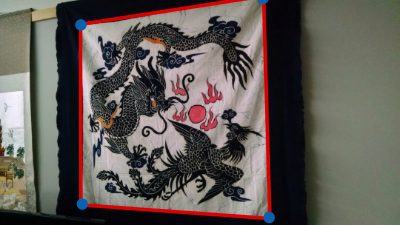
\includegraphics[width=.95\textwidth]{section01/assets/giftbox_1.png}
\subcaption{}
\end{minipage}%
\begin{minipage}[t]{0.5\textwidth}
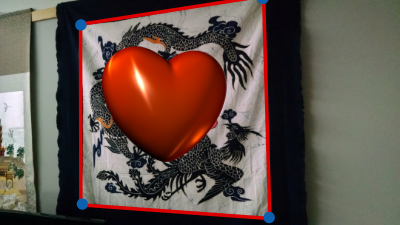
\includegraphics[width=.95\textwidth]{section01/assets/giftbox_2.png}
\subcaption{}
\end{minipage}%
\caption[Short Caption]{Example Result}
\end{figure}

\paragraph{} This application also contains a web interface that allows user to have a general idea of the whole project before they download the android application. Users can not only view and edit their profile but also manage their friends list online. If you don't have your Android device with you it will be a good choice to check if you have any recently received gifts online as well. At the same time, it leaves an interface for administrator users to add more virtual gifts into the database and manage user activities.



}{}\clearpage
\IfFileExists{section02/section}{\section{Requirements}
\label{sec:Requirements}



%openCV, bmob
\subsection{Overview} 
\label{RequirementsOverview}
\paragraph{}
The Gift Box Project was conceived by Dr. Hunt inspired by the very popular game Pokemon Go. For this project, Dr. Hunt served as the supervisor and the sponsor.
\par The supervisor met with the developer several times to gather informal functional requirements of this program. These informal functional requirements helped to define the scope of the program as well as capture the true nature and purpose of the application. During the first of these informal meetings, the supervisor provided samples of the processed pictures with a wall-hanging and identified how to select a region. Based on the information collected from these meetings, the requirement document version 1.0 was created, in which the following requirements were listed:
\begin{itemize}
\item This project will support both a web interface and an Android application.
\item The gifts sent by a user can be selected from a pre-defined library or created by users. 
\item The gift will be projected onto the region chosen by user.
\item GPS navigation allows users to find gifts but it only supports 2D locations. 
\item The application will attempt to robustly allow gifts to be found from a variety of angles, distances, and lighting conditions.
\end{itemize}
\par The project initially included the development of the image comparator which include image recognition and image transformation algorithms. However, the scope of the image comparator was too large and imposed too much complexity on the developer. To address this complexity, the developer, with assistance from Dr. Hunt, decided to use third-party software packages which would be able to perform the functionalities of image recognition. A software package was chosen depending on the required features. The scope of the program was therefore appropriately reduced by using the third-party software for the complex image recognition.
\par The detailed functional requirements are described in Section \ref{FunctionalRequirements} Functional Requirements. 

\subsection{Functional Requirements}
\label{FunctionalRequirements}
\paragraph{}
This program only supports one role, the System User for Android Application. Figure \ref{Use Cases Diagram} gives a Use Case diagram for the System User.
\par As shown in the Figure \ref{Use Cases Diagram}, there are eight use cases in the diagram. Each use case describes a functional requirement. These functional requirements are narrated as follows:

\begin{figure}[htb]
\centering
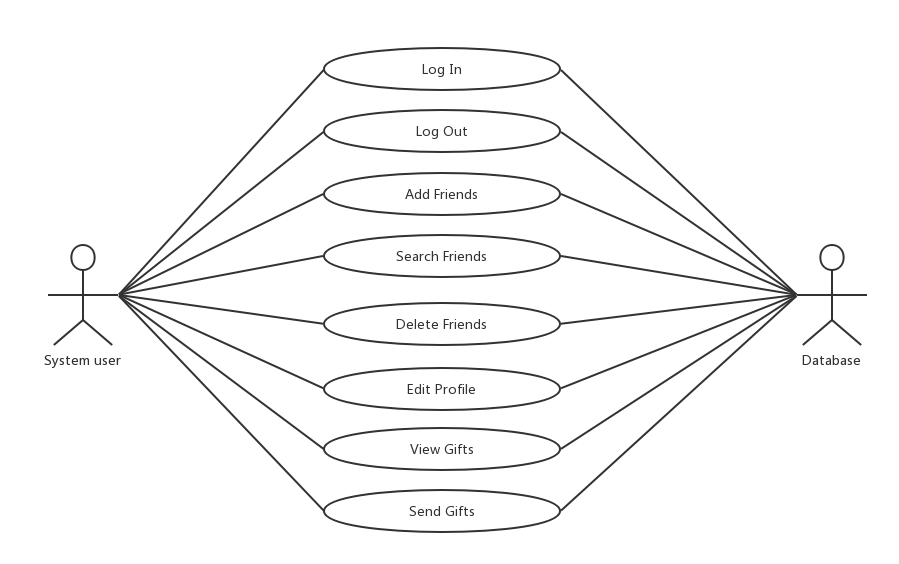
\includegraphics[width=.5\textwidth]{section02/assets/UseCase.png}
\caption[Use Case Diagram for Android Application]{\label{Use Cases Diagram}Use Case Diagram for Android Application}
\end{figure}

\begin{itemize}
\item The \bsq{Log In} function allows users to log in to the system.
\item The \bsq{Log Out} function allows users to log out of the system.
\item The \bsq{Add Friends} function allows users to add other users as friends. This add function doesn't need other users' agreement.
\item The \bsq{Search Friends} function allows users to search other users by username.
\item The \bsq{Delete Friends} function allows users to delete friends from their friends list.
\item The \bsq{Edit Profile} function allows users to edit their password and portrait information. The username and email cannot be changed after registration. 
\item The \bsq{View Gifts} function allows users to view their gifts. Gifts are filtered based on \bsq{Sent} or \bsq{Received}.
\item The \bsq{Send Gifts} function allows users to send virtual gifts to other users.
\end{itemize}
\par The web interface contains the same functionalities as the Android application except for the \bsq{Send Gift} functionality.  Also, the web interface doesn't display those gifts that have not yet been found.
\subsection{Selection of Life Cycle Model}
\paragraph{} At the project inception, we recognized several factors that would affect the development strategy. These factors are listed below.
\begin{itemize}
\item Lack of detailed specification for the GUI.
\item Lack of experience with image recognition.
\item Potential misunderstandings between the project sponsor and the developer.
\end{itemize}
\par To address these factors, we determined to use an adaptive software development model. The adaptive model is a method of software development where the model is designed, implemented and tested incrementally until the product is finished. 
\par Compared to other models, this one will check the consistency between requirements in each iteration. Developers ensure that the product is partially ready with the selected requirements and customers can see the progress of the development process. The graphical illustration of incremental prototyping model is shown in Figure \ref{IncrmentalModel}. In this figure, the `Conventional` line describes the waterfall model where increased functionality generally takes more time to obtain than the incremental approach. The implementation of a new subset of functionalities is obtained quicker in the incremental approach and must be approved by the customer before adding the next subset. This can also be called  the “staircase model”.

\par As a result, each partial functionality can be checked in each interaction and developers will be able to obtain feedback for correcting minor inconsistencies between the delivered product and the user expectations.  Also, if minor alterations to the requirements are indicated, these changes can be addressed within each increment.

\begin{figure}[htb]
\centering
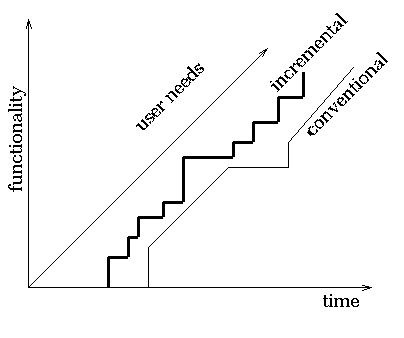
\includegraphics[width=.5\textwidth]{section02/assets/IncrementalModel.png}
\caption[Graphical Illustration of Incremental Prototyping Model]{\label{IncrmentalModel}Graphical Illustration of Incremental Prototyping Model}
\end{figure}

\par Each increment includes the completion of several functional requirements. This project involved seven total increments.  The functional requirements associated with each increment were determined by the sponsor and the developer.  The order in which the requirements for each iteration were determined was dependent upon their general importance and their contribution to the entire system.
\par Functionalities concerning image recognition procedure  and image processing should have a higher priority than others. The increments that occurred in this project are listed below:
\begin{itemize}
\item Increment 1: Graphical User Interface functionalities related to basic user interaction.
\item Increment 2: Image recognition's functionalities related to application interaction.
\item Increment 3: Image perspective functionalities related to application interaction.
\item Increment 4: Enhancing application review and evaluation.
\item Increment 5: System configuration.
\item Increment 6: Writing and executing test cases.
\item Increment 7: Enhancing interactivity of Graphical User Interface.
\end{itemize}}{}\clearpage
\IfFileExists{section03/section}{\section{Design}
\label{sec:Design}

\subsection{Database Design} 
Bmob online database was chosen for the database management system (DBMS) for both the Android application and the web interface because it is a free and open source product. The entity relationship (ER) diagram for the whole project is shown in Figure \ref{ERDiagram}.

\begin{figure}[htb]
\centering
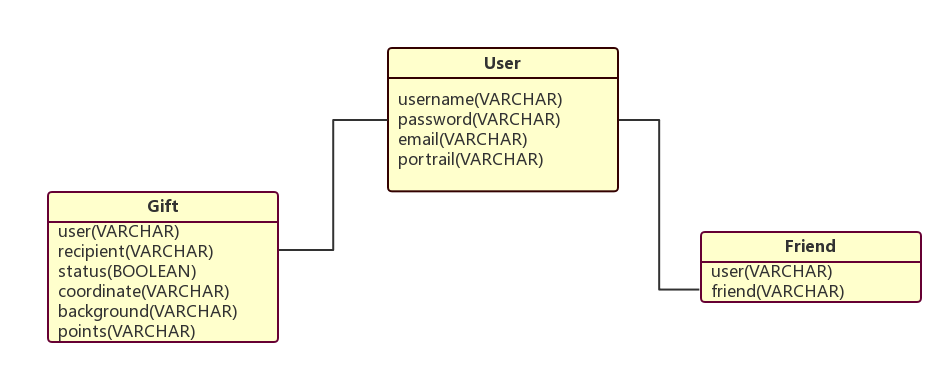
\includegraphics[width=.5\textwidth]{section03/assets/ERDiagram.png}
\caption[Short Caption 2]{\label{ERDiagram}ER Diagram for the project}
\end{figure}

\paragraph{}
All three tables designed for this project are listed in the ER Diagram.
\begin{itemize}
\item The 'User' table will save all the user information. In this table username and email will be unique for each user and this will be verified when users are registered.
\item The 'Friend' table is for saving all friends pairs and both 'user' and 'friend' columns are usernames from 'User' table.
\item The 'Gift' table saves all the gifts information. The 'user' column records the user who sent the gift. The 'recipient' column records the user who will receive the gift. The 'status' column is a boolean type data meaning the gift is found if it is 'true'. The 'coordinate' column is designed to hold the location where the gift was sent. The 'background' column is designed to hold the region picture and the 'points' column is designed to hold the four corners selected by users.
\end{itemize}

\subsection{User Interface Design}
\paragraph{}Following the user interface design principles, especially the accessibility, this user interface is designed to be clear and easy to use. All the parts keep the same color style and try not to use too many colors and fonts so that the user interface is aesthetically pleasing. The main pages are listed below:
\begin{figure}[htb]
\centering
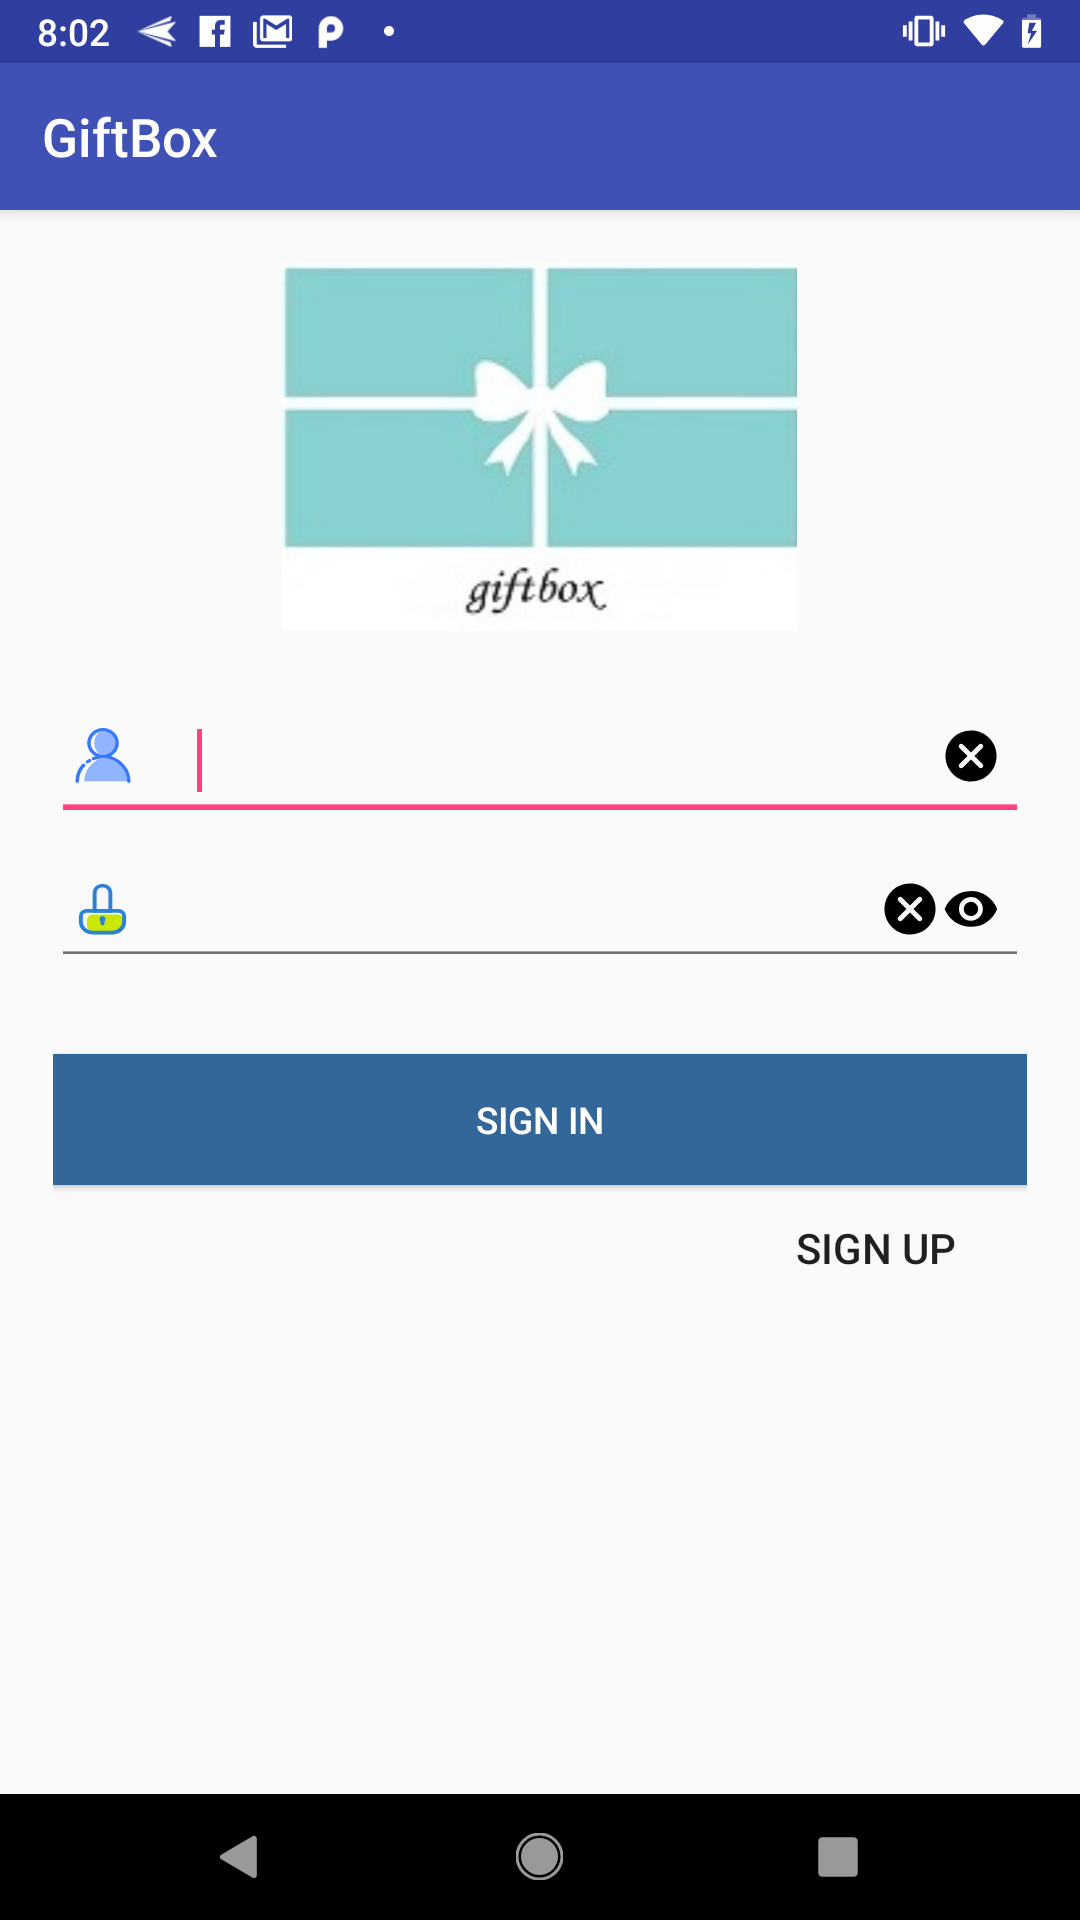
\includegraphics[width=.5\textwidth]{section03/assets/SignIn.png}
\caption[Short Caption 2]{\label{SignInUI}ER Diagram for the project}
\end{figure}
\par The sign in page is shown in Figure \ref{SignInUI}. The logo is designed to show up so that the user will know which application they are using. The user icon and the password icon at the left side of the text field hint the meaning of the two fields to the users. The delete icon and the eye icon at the right side of the text field used another color because they have different functions. Users can use the delete button to delete the whole string they typed in and view the password in plain text or encrypted text. The 'Log In' button is designed to be big to prevent users from making mistakes. 

\begin{figure}[htb]
\centering
\begin{minipage}[t]{0.5\textwidth}
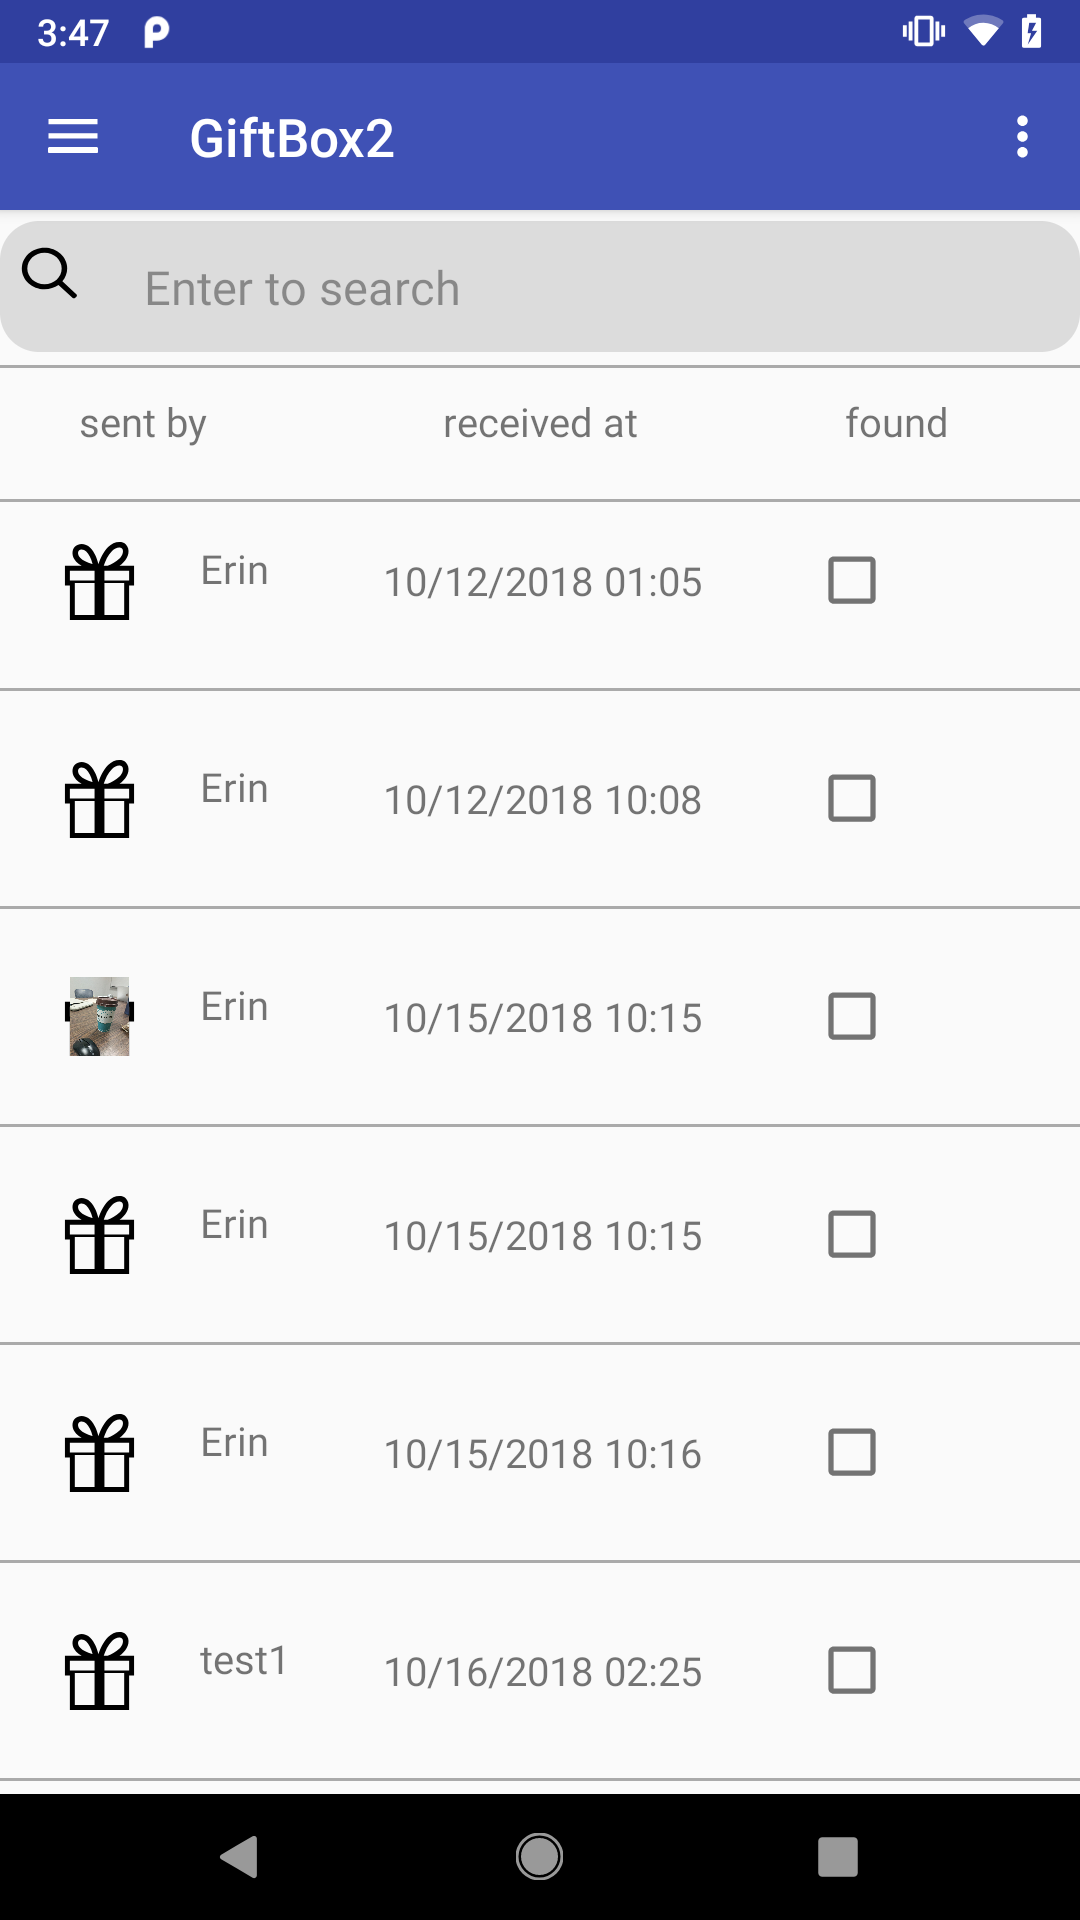
\includegraphics[width=.95\textwidth]{section03/assets/MainPage.png}
\subcaption{\label{GiftsListMainUI}}
\end{minipage}%
\begin{minipage}[t]{0.5\textwidth}
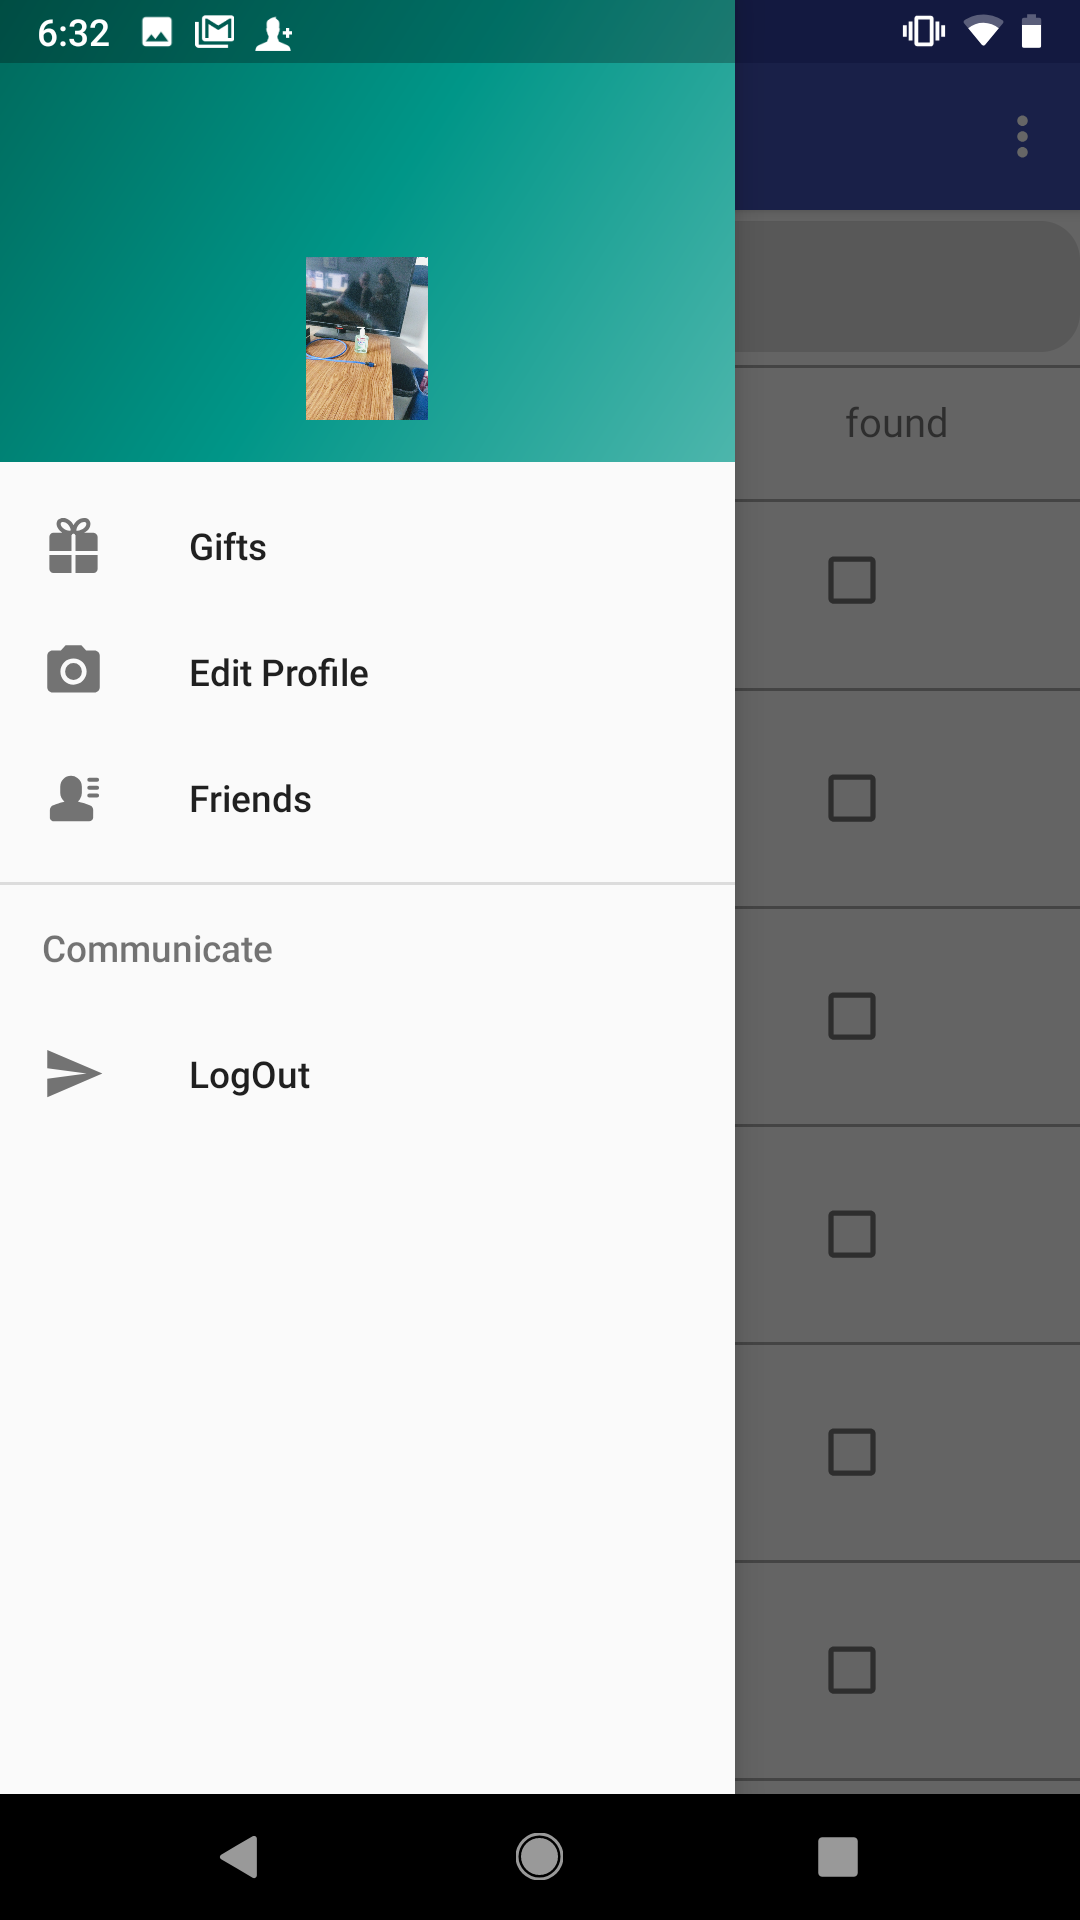
\includegraphics[width=.95\textwidth]{section03/assets/MainPortrait.png}
\subcaption{\label{FunctionsMainUI}}
\end{minipage}%
\caption[Short Caption 2]{\label{MainPageUI}Main page}
\end{figure}
\par The main page is shown in Figure \ref{MainPageUI}. The Figure \ref{GiftsListMainUI} shows the gifts received by the user. The top search field can searched by username. This page also has titles to tell user the meaning of each column. The gift icon was replaced by user portraits later. The found column shows whether or not the gift is found. If the box is checked that means the gift is found.
\par The navigation menu will lead users to other functional pages. Users will see their portraits on the top of this page and will be able to change their portraits by clicking on the profile picture. They can also view their gifts list by clicking on the 'Gifts' button, edit their profile by clicking on the 'Edit Profile' button, view their friends list as shown in Figure \ref{FriendsListUI} by clicking on the 'Friends' button and they will be able to log out from the system by clicking on the 'LogOut' button. 

\begin{figure}[htb]
\centering
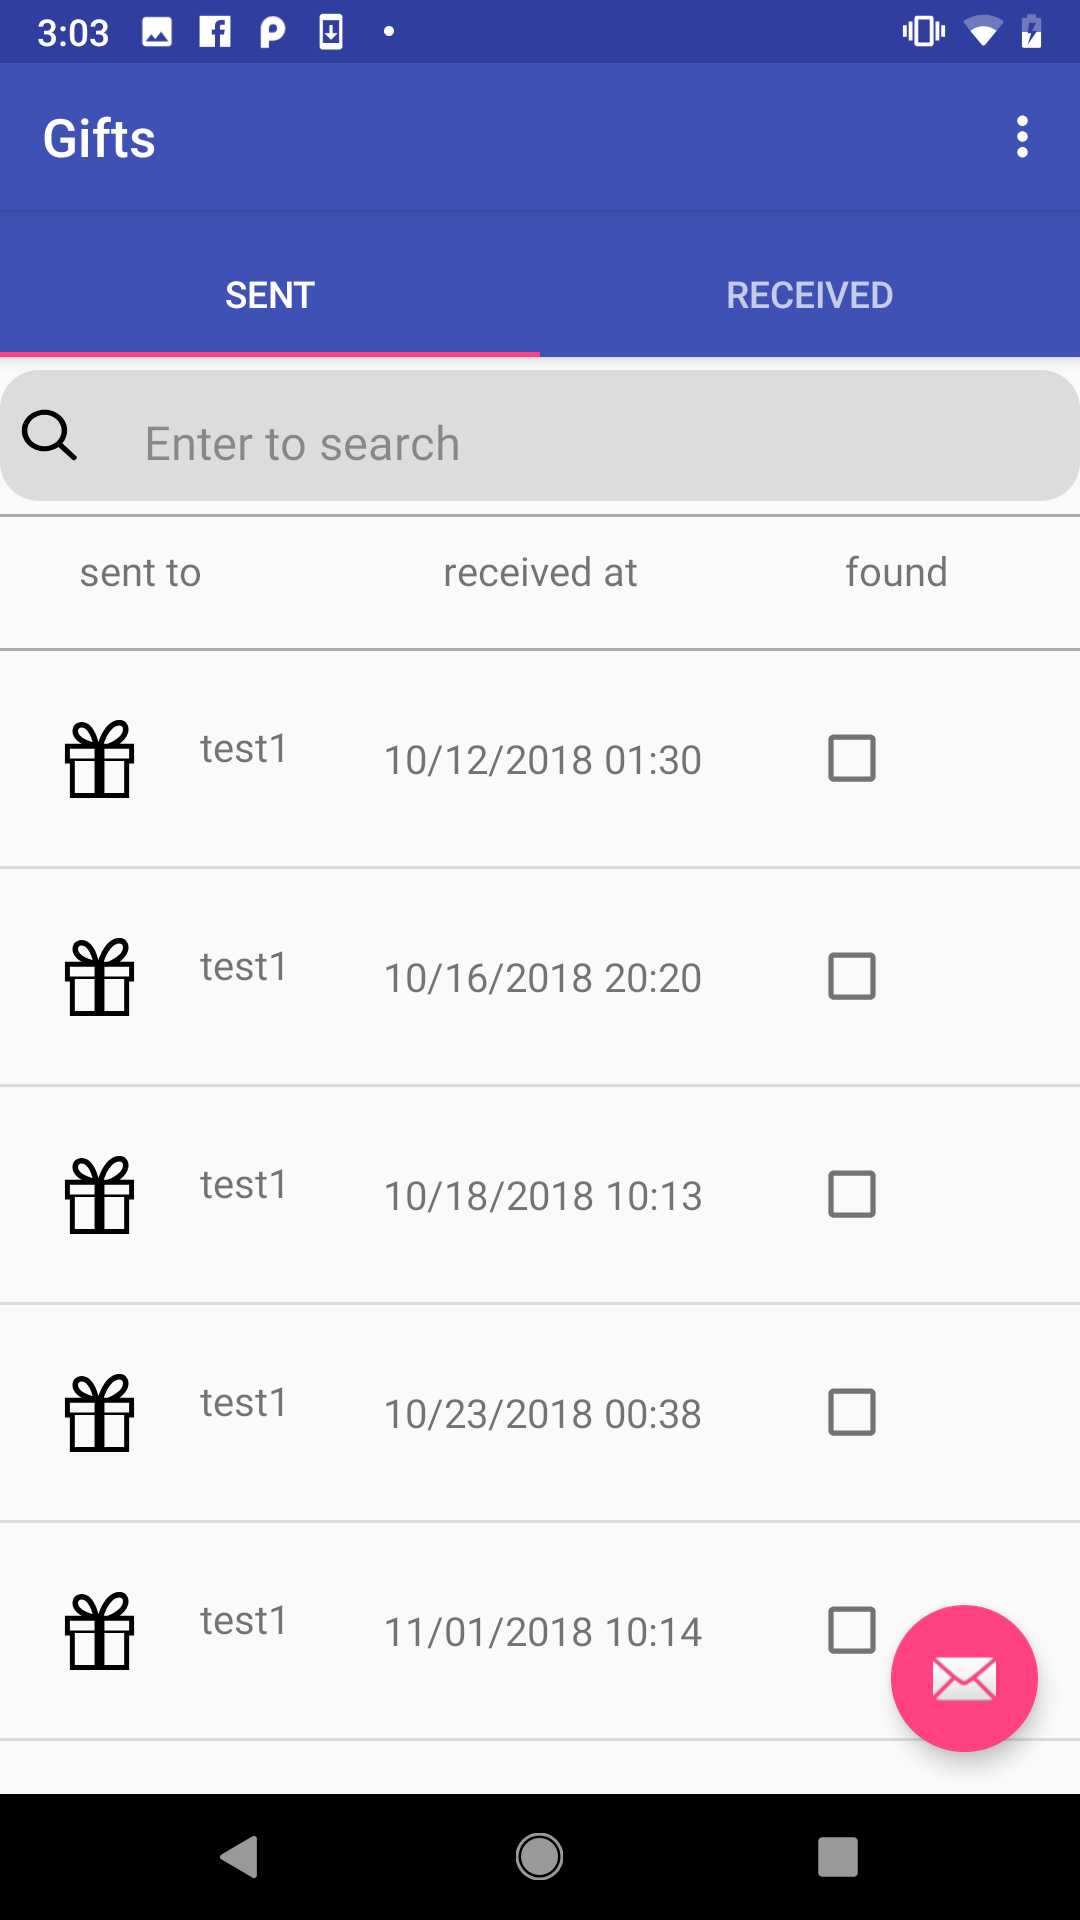
\includegraphics[width=.5\textwidth]{section03/assets/GiftsList.png}
\caption[Short Caption 2]{\label{GiftsListUI}Gifts List page}
\end{figure}
\par Figure \ref{GiftsListUI} is very similar to the main page gifts list but in this page users will be able to see not only received gifts but also sent gifts ordered by time stamp. For the sent gifts, users will be able to see if this gift is found or not by clicking on the gift. For the received gifts, they can only view found gifts and begin to find unfound gifts by clicking on the gift. 


\begin{figure}[htb]
\centering
\begin{minipage}[t]{0.5\textwidth}
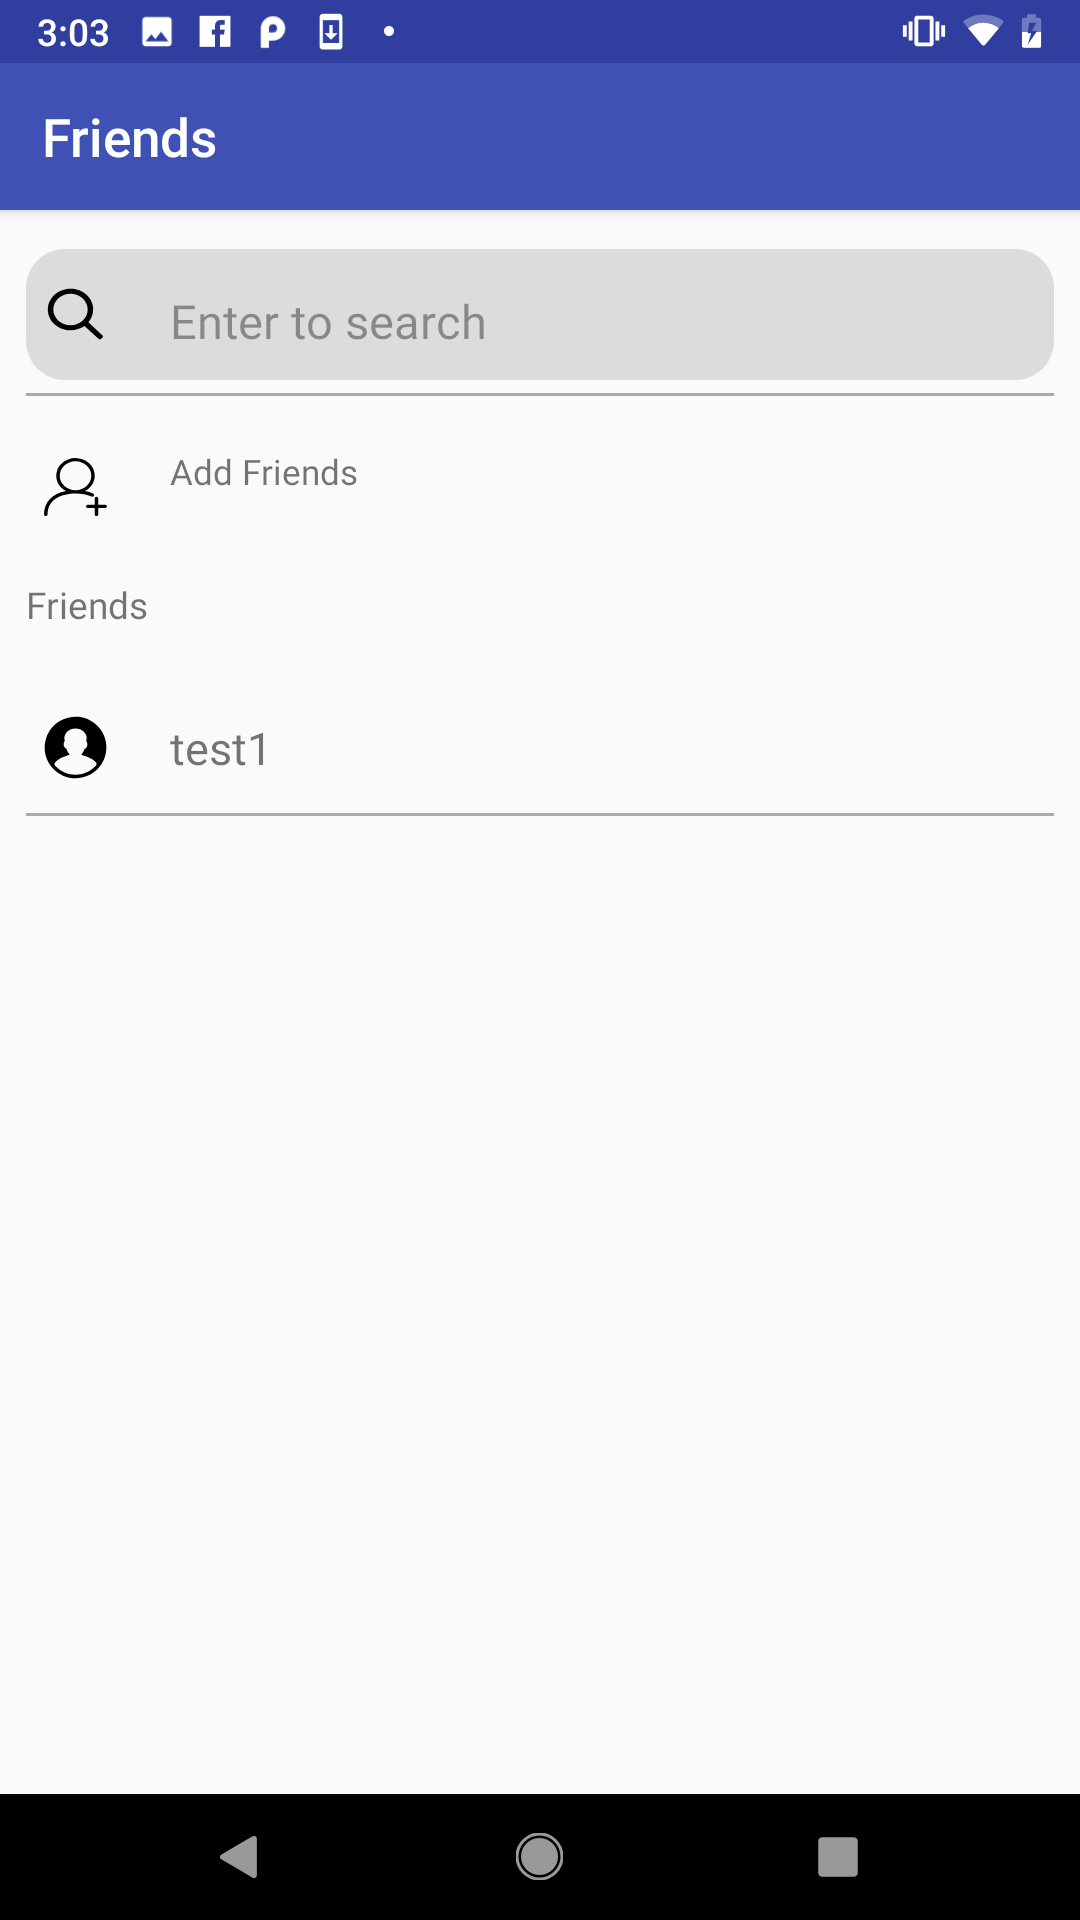
\includegraphics[width=.95\textwidth]{section03/assets/FriendsList.png}
\subcaption{\label{FriendsListUI}}
\end{minipage}%
\begin{minipage}[t]{0.5\textwidth}
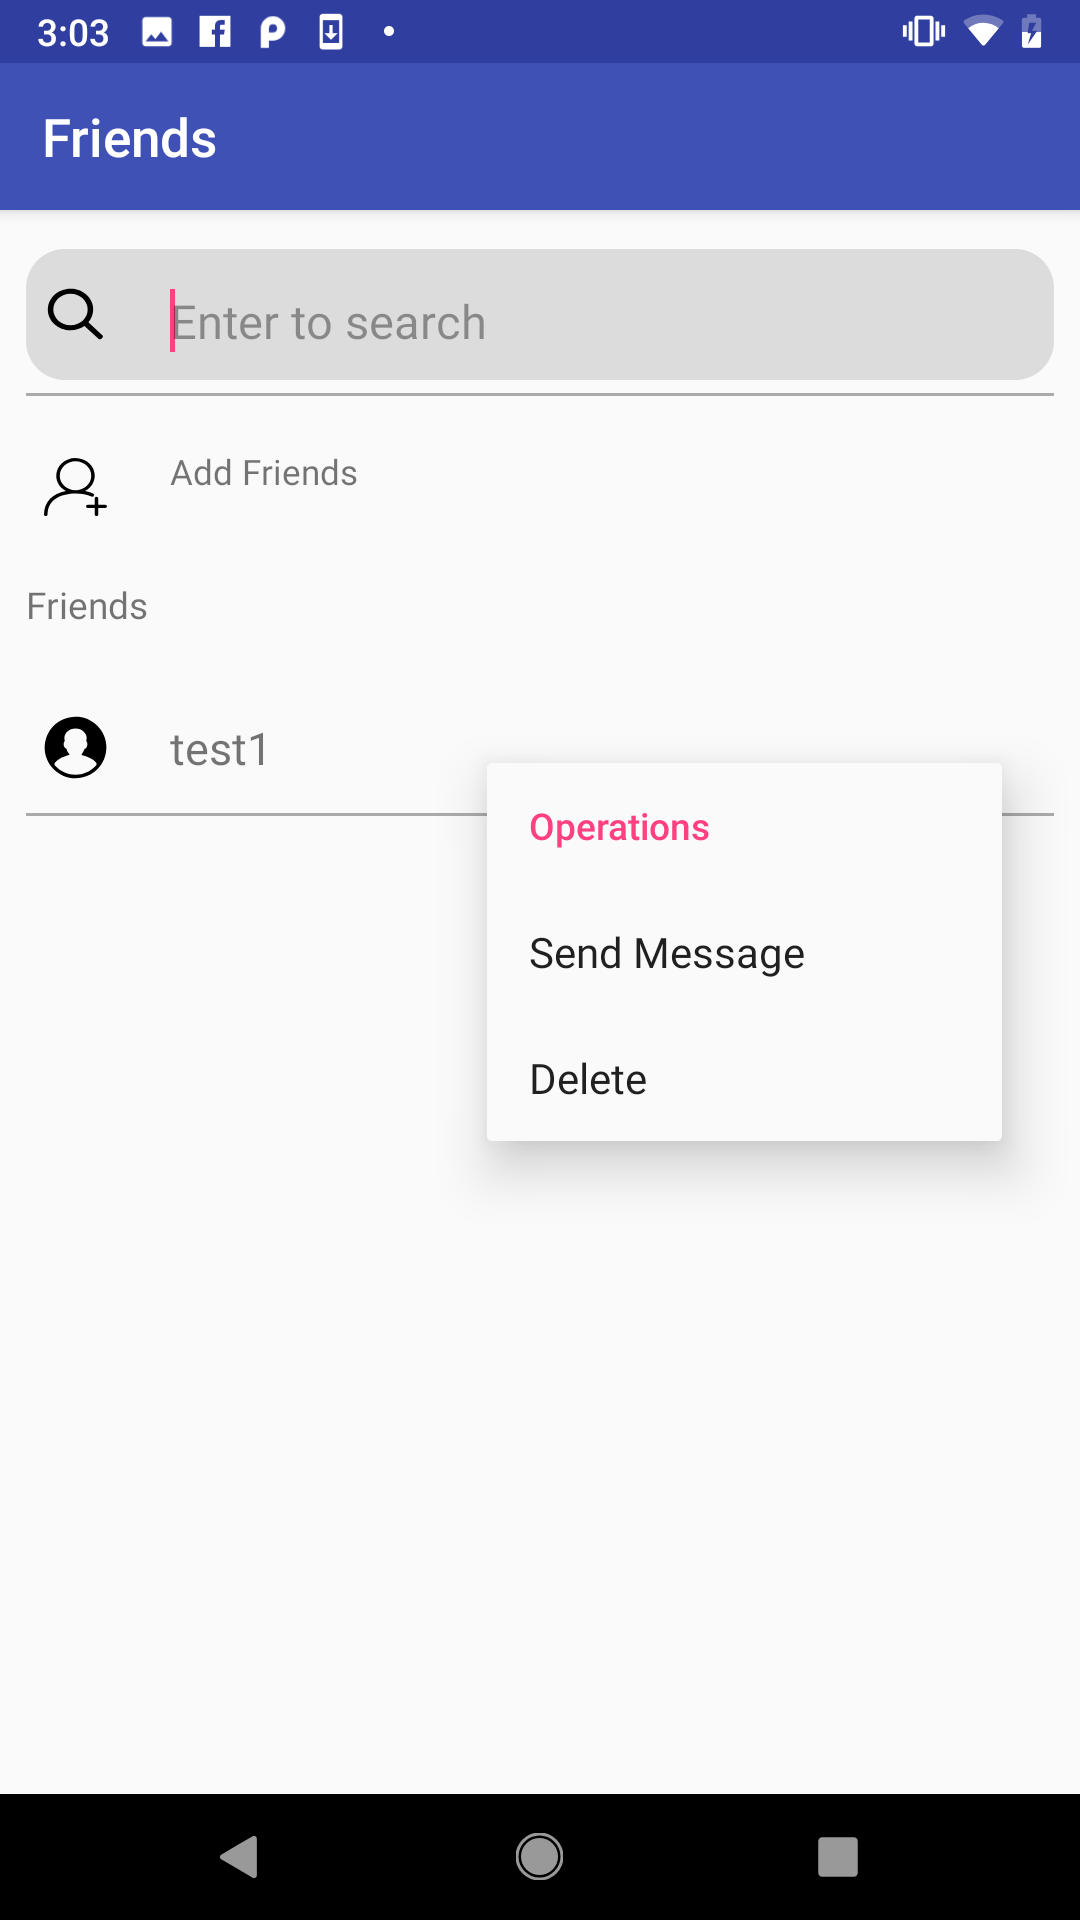
\includegraphics[width=.95\textwidth]{section03/assets/FriendsListAction.png}
\subcaption{\label{FriendsListActionUI}}
\end{minipage}%
\caption[Short Caption 2]{\label{WholeFriendsListUI}Friends List page}
\end{figure}

\par As shown in Figure \ref{WholeFriendsListUI}, the friends list is another important page for this application. To convenience users, the search field can let users search their friends if their friends list is too long. Users can also add friends by clicking on the 'Add Friends' button. The friends list is shown below. Users can get further functions by long clicking on friends' names, as shown in Figure \ref{FriendsListActionUI}. 

\begin{figure}[htb]
\centering
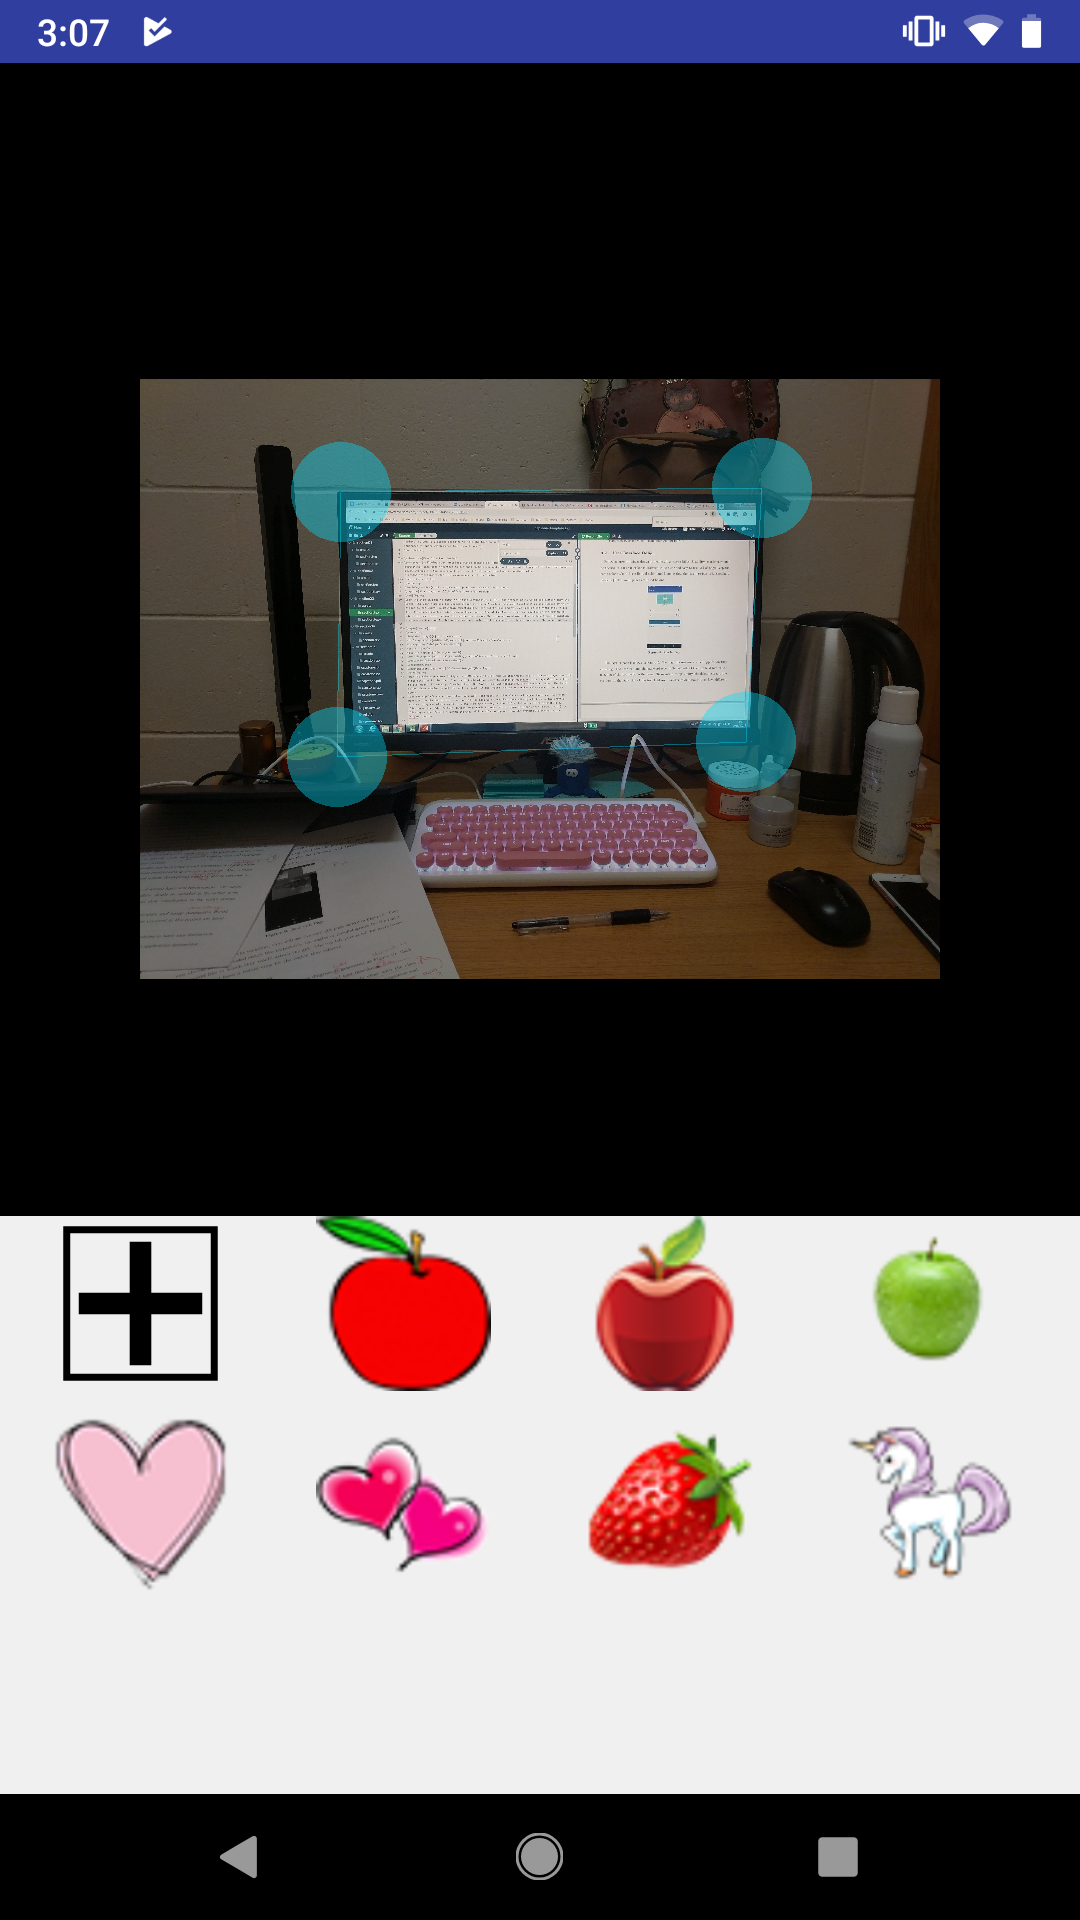
\includegraphics[width=.5\textwidth]{section03/assets/SendGift.png}
\caption[Short Caption 2]{\label{SendGiftUI}Send Gift Page}
\end{figure}
\par After users choose the recipient, they will see the send gift page shown in Figure \ref{SendGiftUI}. They can choose any four sided shape like trapezoids, rectangles or parallelograms for the region they would like in which they would attach the gift.

\subsection{Architecture Design}
\paragraph{}Based on the functional requirements, the class diagram is generated as Figure \ref{ClassDiagram}. Each class is correspond to one or more functional requirements and user interfaces.
\par As we can see, the basic user interaction related class is already clear with the class diagram. So we are just going to explain classes and functions about image recognition and navigation.

\begin{figure}[H]
\centering
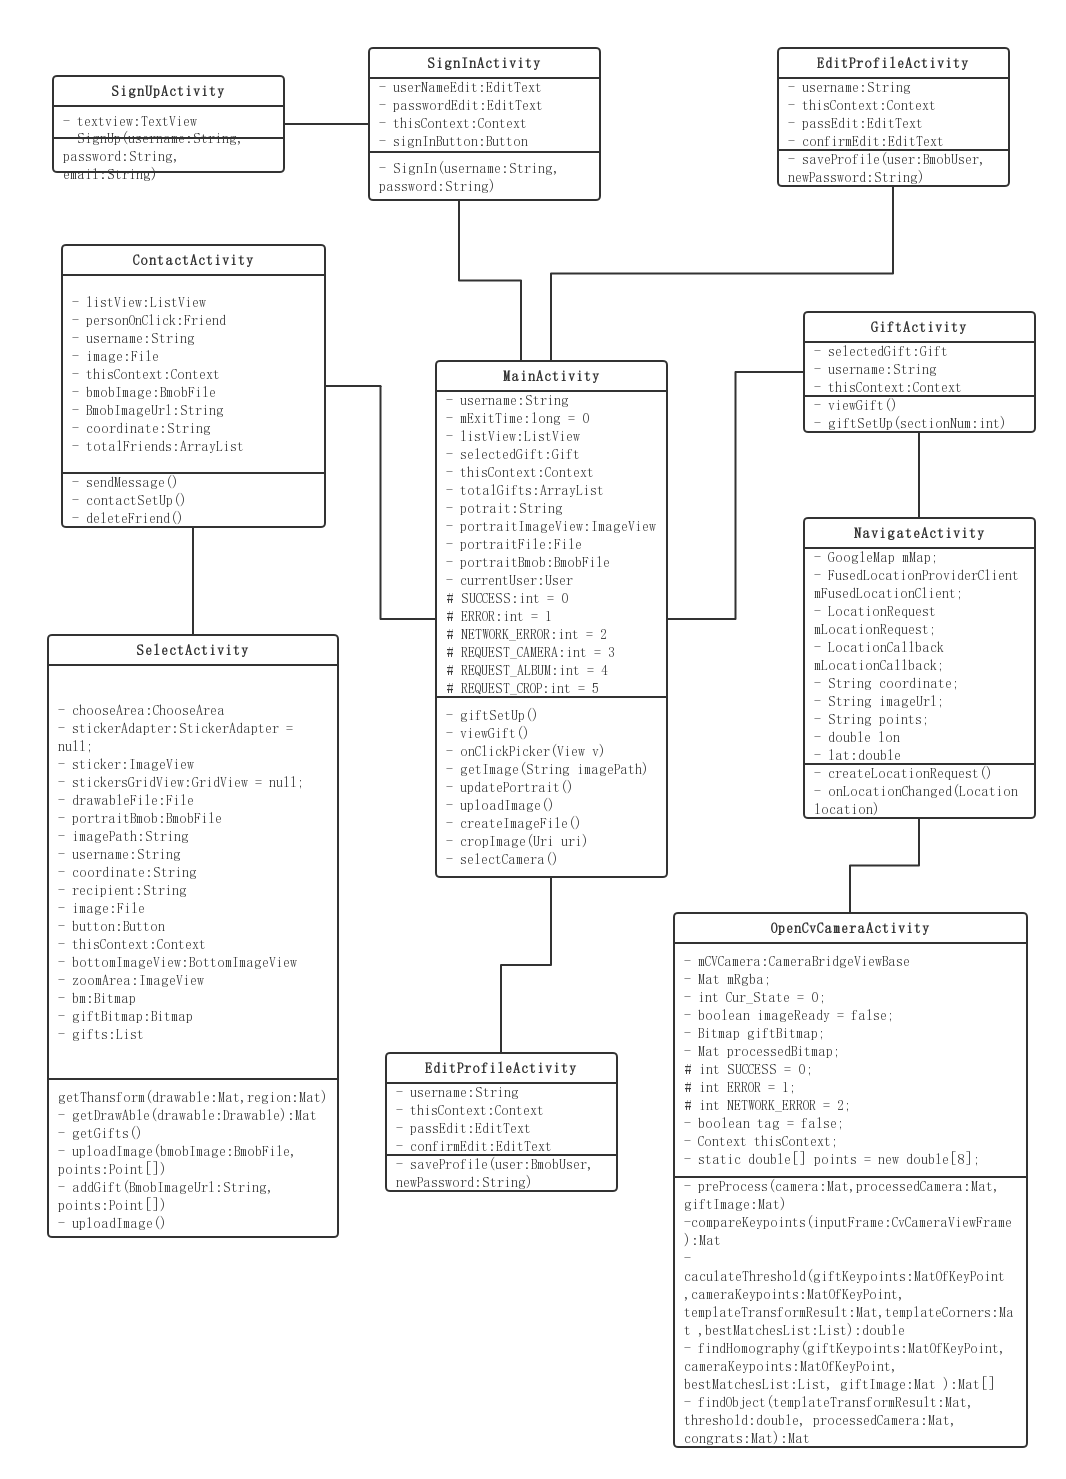
\includegraphics[width=.8\textwidth]{section03/assets/ClassDiagram.png}
\caption[Short Caption 2]{\label{ClassDiagram}Class Diagram}
\end{figure}
\par The 'ContactActivity' is mainly related to the user interface shown in Figure \ref{FriendsListUI}, users will be able select their recipient and the information will be taken to 'SelectActivity' by an intent and then the system camera will be called to get the background image, the 'chooseArea' attribute is an instance of helper class 'ChooseArea' to let the users choose the region. After that, the gift will fit in the region by 'getTransform' method and 'addGift' method will save all the information to the database.
\par The receiving process is explained as follow. The 'GiftActivity' is designed to show the gift list which shown in Figure \ref{GiftsListUI}, when users click on a not found gift they will go to 'NavigationActivity'. The 'NavigationActivity' is designed to manage user locations and Google Map activities. Users will be able to see their location on the map and the gift location will be marked in a red point. When user found where the gift locates, the real-time image recognition will start. The camera capture images will compare with the database saved background image. The 'preProcess' method is used to download the database saved background image and resize the camera capture image. The 'compareKeypoints' method calculates the keypoints in two images and find the matches. The 'findHomography' method will use the matches found before to generate the homography and perform a perspective transformation on the template image to correct the image to get the region in camera image. But this method cannot always get the correct result, so the 'caculateThreshold' method calculate the value of the number of keypoints not in selected region divide the number of keypoints in detected region, this value will be later used as a threshold to determine if the region we found is good. At last, the 'findObject' method will get the final detected region and show the gift on it.


}{}\clearpage
\IfFileExists{section04/section}{\section{Implementation}												
\label{sec:Implementation}

\paragraph{}For the Android application, Android and Java were chosen as the primary programming languages due to the developer's familiarity with them. For the web interface, JSP was chosen as the background language. JavaScript and HTML were chosen to take care of the front-end and user interface. Ajax is also used to talk to the database. 

\subsection{Database Operations}
\label{subsec:DatabaseOperations}
\paragraph{}As what we mentioned in the design section, the Bmob online database was chosen for the database management system (DBMS) for both the Android application and the web interface. To use this database, we need an entity class to match each form. The entity class will extends BmobObject and the class name must be the same as the form name. As shown below:
\begin{lstlisting}[language={java},
        numbers=left,basicstyle=\small\ttfamily]
public class Friend extends BmobObject {
    private String user;
    private String friend;
    public String getUser() {
        return user;
    }
    public void setUser(String user) {
        this.user = user;
    }
    public String getFriend() {
        return friend;
    }
    public void setFriend(String friend) {
        this.friend = friend;
    }
}
\end{lstlisting} 
\begin{figure}[htb]
\centering
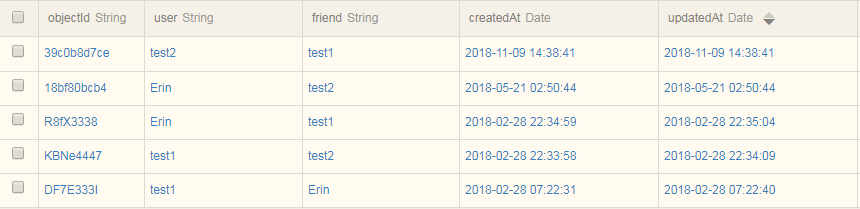
\includegraphics[width=.9\textwidth]{section04/assets/databaseOverview.png}
\caption[Short Caption]{\label{DatabseOverview}Form 'Friend'}
\end{figure}
\par Figure \ref{DatabseOverview} is the corresponding form in the database. The 'objectId', 'createdAt' and 'updatedAt' columns are generated by Bmob automatically. 
\par After we got the entity classes, we can begin to initialize. Three steps are needed for the initialization: 
\begin{enumerate}
\item[1)]Import SDK into your app level build.gradle file like this:
\begin{lstlisting}[language=JAVA] 
implementation 'cn.bmob.android:bmob-sdk:3.6.3'
\end{lstlisting} 
\item[2)] Configure AndroidManifest.xml file. This file is used to declare an application component and declare the permissions that the application needs. We will include this in later subsection \ref{subsubsec:GetSystemPermissions} Get System Permissions.
\item[3)] Initialize BmobSDK like the code shown below. The 'this' means the context and the 'ApplicationID' is defined when creating the project on Bmob website. The 'ApplicationID' is only accessible by the developer which maintains the security.
\begin{lstlisting}[language=JAVA] 
Bmob.initialize(this, "Your Application ID");
\end{lstlisting} 
\end{enumerate}
\par After initialization is finished. We can get access to the database like this:
\begin{lstlisting}[language={java},
        numbers=left,basicstyle=\small\ttfamily]
BmobQuery<User> query = new BmobQuery<>();
query.addWhereEqualTo("username", username);
query.findObjects(new FindListener<User>() {
    @Override
    public void done(List<User> users, BmobException e) {
        if(e == null){
            saveProfile(users.get(0),newPassword);
        }else{
            Log.i("bmob","failed:"+e.getMessage()+","+
            e.getErrorCode());
        }
    }
});
\end{lstlisting} 
\par All the data operations have a template which makes it easier to perform database operations.An inner class will be needed for each database operation. This piece of code shows how to retrieve data. Line 2 adds a constraint for the query which is the value of 'username' column equals the String username. The users in Line 5 will save the result if the query succeeded. If the error message, e, is null, then it means the query succeeded. 
\subsection{Image Processing Algorithms}
\paragraph{}This project addresses two central problems about image processing: transform the virtual gift to fit in user selected regions and find the correct region when user receive the gift. 

\subsubsection{Gift Transformation}
\paragraph{} Gift transformation is applies a perspective transformation of one image to another image. For perspective transformation, we need a 3x3 transformation matrix. Straight lines will remain straight even after the transformation. To find this transformation matrix, we need four points on the gift image which will be the four corners of the gift image and corresponding points on the background image. The corresponding points will be the four corners of the user selected region.  Among these four points, three of them should not be collinear. Then transformation matrix can be found by the function getPerspectiveTransform at Line 15. Then use the warpPerspective function at Line 16  to apply transformation with this 3x3 transformation matrix. The code below is the method used to apply transformation, drawable is the gift image, region is the background image, points contains the four corners user selected.
\begin{lstlisting}[language={java},
        numbers=left,basicstyle=\small\ttfamily,breaklines=true]
public Mat getThansform(Mat drawable, Mat region, int[] points) {
    Mat drawableCorner = new Mat(4, 1, CvType.CV_32FC2);
    Mat drawableTransformCorner = new Mat(4, 1, CvType.CV_32FC2);

    drawableCorner.put(0, 0, new double[]{0.0, 0.0});
    drawableCorner.put(1, 0, new double[]{drawable.cols(), 0.0});
    drawableCorner.put(2, 0, new double[]{drawable.cols(), drawable.rows()});
    drawableCorner.put(3, 0, new double[]{0.0, drawable.rows()});
    
    for(int i=0; i<4; i++){
        drawableTransformCorner.put(i, 0, new double[]{points[i*2], points[i*2+1]});
    }

    Mat perspectiveTransform = Imgproc.getPerspectiveTransform(drawableCorner, drawableTransformCorner);
    Imgproc.warpPerspective(drawable,region,perspectiveTransform, region.size(), Imgproc.INTER_LINEAR,
    Core.BORDER_TRANSPARENT, new Scalar(0, 0, 0, 0));

    return region;
}
\end{lstlisting} 
\subsubsection{Region Recognition}
\paragraph{}Image recognition is more complex, we used 'Features2D' and 'Homography' in OpenCv to find a known object in a real time camera capture frame. 'Features2D' and 'Homography' are all come from the third party library, OpenCV. OpenCV is a cross-platform library which we can use to develop real-time computer vision applications. It mainly focuses on image processing, video capture and analysis including features like face detection and object detection. For this project we mainly use the 'Features2D' class to find keypoints and matches. Then use 'Homography' to determine the object.
\par Before we begin to detect image features, we need to have a pre-process to call the camera so that we can get each frame to be compared. This will be introduced in Section \ref{CallCamera} Call Camera. The steps and corresponding code to recognize region are listed below:
\begin{enumerate}
\item[1)] Detect the keypoints using AKAZE Detector. AKAZE is a novel and fast multiscale feature detection and description approach that exploits the benefits of nonlinear scale spaces.\cite{alcantarilla2011fast} This piece of code put the ProcessedCamera image keypoints into cameraKeypoints. 'FeatureDetector' is an OpenCv class used to generate different feature detectors. 'MatOfKeyPoint' is a matrix used to save keypoints.
\begin{lstlisting}[language={java},
        numbers=left,basicstyle=\small\ttfamily,breaklines=true]
FeatureDetector featureDetector = FeatureDetector.create(FeatureDetector.AKAZE);
MatOfKeyPoint cameraKeypoints = new MatOfKeyPoint();
Imgproc.cvtColor(processedCamera, processedCamera, Imgproc.COLOR_RGBA2RGB);
featureDetector.detect(processedCamera, cameraKeypoints);
\end{lstlisting} 
\item[2)] Calculate descriptors (feature vectors). We get cameraDescriptor for processedCamera here. According to an extensive evaluation based on the standard Oxford benchmark \cite{mikolajczyk2005} that shows the excellent compromise between speed and performance of our approach compared to state-of-the-art methods such as BRISK, ORB, SURF, SIFT and KAZE. While A-KAZE is more expensive to compute than BRISK and ORB, it is faster than SURF, SIFT and KAZE.\cite{alcantarilla2011fast}
\begin{lstlisting}[language={java},
        numbers=left,basicstyle=\small\ttfamily,breaklines=true]
DescriptorExtractor extractor = DescriptorExtractor.create(DescriptorExtractor.AKAZE);
Mat cameraDescriptor = new Mat();
extractor.compute(processedCamera, cameraKeypoints, cameraDescriptor);
\end{lstlisting} 
\item[3)] Matching descriptor vectors using 'BRUTEFORCE\_HAMMING' matcher and only save 'good' matches, the smaller the distance the better the match and here we only use the first half of the matches. 
\begin{lstlisting}[language={java},
        numbers=left,basicstyle=\small\ttfamily,breaklines=true]
MatOfDMatch matches = new MatOfDMatch();
DescriptorMatcher matcher = DescriptorMatcher.create(DescriptorMatcher.BRUTEFORCE_HAMMING);
matcher.match(cameraDescriptor, giftDescriptor, matches);
            
List<DMatch> bestMatchesList = mats.stream().filter( m -> (m.distance - MIN_DIST) < .5 * range)
                    .collect(Collectors.toList());
\end{lstlisting} 
\item[4)] Get the keypoints from the 'good' matches. 'bestMatchesList' is a List of 'DMatch'. 'DMatch' is a data type used to save a match in OpenCv and each 'DMatch' will have the following attributes:
\begin{itemize}
\item distance: This attribute gives us the distance between the descriptors. A lower distance indicates a better match.
\item trainIdx: This attribute gives us the index of the descriptor in the list of train descriptors (in our case, it’s the list of descriptors in the gift images).
\item queryIdx: This attribute gives us the index of the descriptor in the list of query descriptors (in our case, it’s the list of descriptors in the camera capture images).
\item imgIdx: This attribute gives us the index of the train image. 
\end{itemize}
\paragraph{} In our case, we just need first three attributes. The following code shows how we save keypoints into a LinkedList, 'objectPoints' will save the gift image keypoints and 'scenePoints' will save the camera capture images keypoints. After we get the keypoints, we will use them to generate the 'homography'. The 'findHomography' method will find a perspective transformation between two planes. The four parameters used in this method are:
\begin{itemize}
\item srcPoints: Coordinates of the points in the original plane, a matrix of the type CV\_32FC2 or vector\textless Point2f\textgreater.(in our case,it's objMatOfPoint2f which comes from gift images)
\item dstPoints: Coordinates of the points in the target plane, a matrix of the type CV\_32FC2 or a vector\textless Point2f\textgreater .(in our case,it's scnMatOfPoint2f which comes from camera capture images)
\item method: Method used to compute a homography matrix.(There are three supported methods, we used RANSAC-based robust method here)
\item ransacReprojThreshold: Maximum allowed reprojection error to treat a point pair as an inlier (used in the RANSAC method only). If srcPoints and dstPoints are measured in pixels, it usually makes sense to set this parameter somewhere in the range of 1 to 10.(in our case, it's three)
\end{itemize}

\begin{lstlisting}[language={java},
        numbers=left,basicstyle=\small\ttfamily,breaklines=true] 
List<KeyPoint> templateKeyPointList = giftKeypoints.toList();
List<KeyPoint> originalKeyPointList = cameraKeypoints.toList();
LinkedList<Point> objectPoints = new LinkedList();
LinkedList<Point> scenePoints = new LinkedList();
    for(int i=0; i<bestMatchesList.size(); i++){
        objectPoints.addLast(templateKeyPointList.get(bestMatchesList.get(i).trainIdx).pt);
        scenePoints.addLast(originalKeyPointList.get(bestMatchesList.get(i).queryIdx).pt);
    }
MatOfPoint2f objMatOfPoint2f = new MatOfPoint2f();
objMatOfPoint2f.fromList(objectPoints);
MatOfPoint2f scnMatOfPoint2f = new MatOfPoint2f();
scnMatOfPoint2f.fromList(scenePoints);
Mat homography = Calib3d.findHomography(objMatOfPoint2f, scnMatOfPoint2f, Calib3d.RANSAC, 3);
\end{lstlisting} 
\item[5)] Put the four corners from the selected region into the template image, in our case, the gift image. Here we use a Mat with one column and four rows to record the points. The 'points' is an array of String with user selected region information retrieved from the database, and then, use perspectiveTransform method which performs the perspective matrix transformation of vectors. There are three attributes for this method: 
\begin{itemize}
\item src: Input two-channel or three-channel floating-point array; each element is a 2D/3D vector to be transformed. (in our case, it's templateCorners which comes from gift image.)
\item dst: Output array of the same size and type as src.(in our case, it's templateTransformResult which will save detected corners)
\item m – 3x3 or 4x4 floating-point transformation matrix.(in our case, it's the homography we generated in last step)
\end{itemize}
\paragraph{} After these operations, four corners will be detected to localize the object. The four detected corners of the region is now saved in templateTransformResult.
\begin{lstlisting}[language={java},
        numbers=left,basicstyle=\small\ttfamily,breaklines=true]
Mat templateCorners = new Mat(4, 1, CvType.CV_32FC2);
Mat templateTransformResult = new Mat(4, 1, CvType.CV_32FC2);
for(int i=0; i<4; i++){
    templateCorners.put(i, 0, new double[]{points[i*2], points[i*2+1]});
}
Core.perspectiveTransform(templateCorners, templateTransformResult, homography);
\end{lstlisting} 
\end{enumerate}
\par When we first finished the code above, we found out several conditions that could be optimized and we tried to add some factors to constrain the object detected. We put two images in a line and use four-sided shapes to draw both the region selected by user and region detected by the algorithm, after testing thousands of different scenes and manual observation, the factors used to optimize the region are listed below:
\begin{enumerate}
\item[1)] If one of the four corners detected is out of the image bound, that result will be abandoned. 
\item[2)] In case an object matches a very small picture which is not the same, for example, a white board with some lines on it matches a tiny white dot, we add a radio to control the detected object's size. The aspect ratio of the detected region must be greater than or equal to point five times the aspect ratio of  the selected region and the aspect ratio of the detected region must be less than or equal to two times the aspect ratio of the selected region.
\item[3)] The third factor we used is the value of the number of keypoints not in the selected region divided by the number of keypoints in the detected region and both keypoints get from the matches. The smaller factor means a better result. After testing, we decided we only want the result when the factor is less than point three. This factor helps to localize the object.
\end{enumerate}

\subsection{Android Application}
\subsubsection{Usage of Adapter}
\paragraph{}
An Adapter object acts as a bridge between an AdapterView (e.g. ListView, Spinner, and GridView) and the underlying data for that view. The Adapter provides access to the data items. The Adapter is also responsible for making a View for each item in the data set. For this project, ListView is used to show friends list and gifts list shown in Figure \ref{FriendsListUI} Friends List page and Figure \ref{GiftsListUI} Gifts List page. GridView is used to show the gifts selection after users choose a region. 

\subsubsection{Get system permissions}
\label{subsubsec:GetSystemPermissions}
\paragraph{} As mentioned in Section \ref{subsec:DatabaseOperations} Database Operations, we need to configure AndroidManifest.xml file. This file is used to declare an application component and declare the permissions that the application needs. As shown below, Line 1 is used to get the internet permission, Line 2 is used to get the external storage permission, and Line 3 is needed to create BmobInstallation. Line 4 is to acquire the system camera permission, we will need this when users send a gift and when users find a gift. Line 5 is used to get user locations. Android offers two location permissions: ACCESS\_COARSE\_LOCATION and ACCESS\_FINE\_LOCATION. The permission you choose determines the accuracy of the location returned by the API. If you specify ACCESS\_COARSE\_LOCATION, the API returns a location with an accuracy approximately equivalent to a city block. However, 'ACCESS\_FINE\_LOCATION' allows an app to access precise location.
\begin{lstlisting}[language={java},
        numbers=left,basicstyle=\small\ttfamily,breaklines=true] 
<uses-permission android:name="android.permission.INTERNET" />
<uses-permission android:name="android.permission.WRITE_EXTERNAL_STORAGE" />
<uses-permission android:name="android.permission.READ_PHONE_STATE" />
<uses-permission android:name="android.permission.CAMERA" />
<uses-permission android:name="android.permission.ACCESS_FINE_LOCATION" />
\end{lstlisting} 
\par The other usage of this file is define an Activity, the code below shows an example. In this example, the Acitivity is named 'SignInActivity' and it is a launcher for this application.
\begin{lstlisting}[language={java},
        numbers=left,basicstyle=\small\ttfamily,breaklines=true] 
<activity
    android:name=".SignInActivity"
    android:label="@string/title_activity_sign_in">
    <intent-filter>
        <action android:name="android.intent.action.MAIN" />
        <category android:name="android.intent.category.LAUNCHER" />
    </intent-filter>
</activity>
\end{lstlisting} 

\subsubsection{Call Camera}
\label{CallCamera}
\paragraph{} The Camera is another important part in this project. There are two functions which use camera: 'Send a gift' and 'Receive a gift'.
For 'Send a gift' we used system camera. Other than get user permissions mentioned in section \ref{subsubsec:GetSystemPermissions} Get System Permissions, this chunk of code shows an example of calling the system camera. Line 2 to Line 8 creates a file in storage. Line 12 called the system camera and Line 20 saved the picture into the system album. In Line 15 we have a check for sdk version, that is because if the targetSdkVersion >= 24, then we have to use FileProvider class to give access to the particular file or folder to make them accessible for other apps. FileProvider is a special subclass of ContentProvider that facilitates secure sharing of files associated with an app by creating a 'content:// Uri' for a file instead of a 'file:/// Uri'. A content URI allows you to grant reading and writing access using temporary access permissions. 
\begin{lstlisting}[language={java},
        numbers=left,basicstyle=\small\ttfamily,breaklines=true] 
private void sendMessage() {
    File mediaStorageDir = new File(Environment.getExternalStoragePublicDirectory(
            Environment.DIRECTORY_PICTURES), "giftbox");
    if (!mediaStorageDir.exists()) {
        if (!mediaStorageDir.mkdirs()) {
            Log.d("GiftBox", "failed to create directory");
        }
    }
    String timeStamp = new SimpleDateFormat("yyyyMMdd_HHmmss").format(new Date());
    image = new File(mediaStorageDir.getPath() + File.separator +
            "IMG_" + timeStamp + ".jpg");
    Intent intent = new Intent(MediaStore.ACTION_IMAGE_CAPTURE);
    intent.addCategory(Intent.CATEGORY_DEFAULT);
    Uri uri;
    if (Build.VERSION.SDK_INT >= Build.VERSION_CODES.N) {
        uri = FileProvider.getUriForFile(thisContext, BuildConfig.APPLICATION_ID+".fileprovider", image);//BuildConfig.APPLICATION_ID + ".fileProvider"
    } else {
        uri = Uri.fromFile(image);
    }
    intent.putExtra(MediaStore.EXTRA_OUTPUT, uri);
    startActivityForResult(intent, 0);
}
\end{lstlisting} 
\par After this we will be able to get the result in onActivityResult method. For 'Receive a gift' we use OpenCv to manage the real-time image processing. Other than what we did to get system camera, the extra steps are shown below:
\begin{enumerate}
\item[1)] Extends CvCameraViewListener2 interface in order to use Java API in OpenCv to get the camera preview. There are three methods need to be implemented: onCameraViewStarted, onCameraViewStopped and onCameraFrame. All the important image processing process will be done in onCameraFrame. In our case, this is the place we finish the region recognition.
\item[2)] Add components that display camera content to the interface layout file. Here we will need JavaCameraView to get and display the preview. opencv:show\_fps="true" and opencv:camera\_id="any" options enable FPS message and allow to use any camera on device. Application tries to use back camera first.The following code shows how to do it.
\begin{lstlisting}[language={java},
        numbers=left,basicstyle=\small\ttfamily,breaklines=true] 
<org.opencv.android.JavaCameraView
    android:id="@+id/camera_view"
    android:layout_width="fill_parent"
    android:layout_height="fill_parent"
    opencv:camera_id="any"
    opencv:show_fps="true" />
\end{lstlisting}
\item[3)] Declare a CameraBridgeViewBase object to hold the JavaCameraView component in layout file and implement binding and add event listener in OnCreate method. OnCreate method is where we used to initialize the activity.
\begin{lstlisting}[language={java},
        numbers=left,basicstyle=\small\ttfamily,breaklines=true] 
CameraBridgeViewBase mCVCamera;
mCVCamera = (CameraBridgeViewBase) findViewById(R.id.camera_view);
mCVCamera.setCvCameraViewListener(this);
\end{lstlisting}
\item[4)] Implement the functions we mentioned above. The 'onCameraViewStarted' method is used to initialize the preview images. The 'onCameraViewStopped' will release resources so that the application won't crash. The 'onCameraFrame' method will take care of all image processing, this method will be called every time camera frame refreshed. But because of the algorithm execute takes time so the project result won't be able to show every frame in the result. 'Cur\_State' is used to monitor if the image process begins. 'imageReady' is to ensure the target image is downloaded from database. 'tag' is used to check if the object has been found.
\begin{lstlisting}[language={java},
        numbers=left,basicstyle=\small\ttfamily,breaklines=true] 
@Override
public void onCameraViewStarted(int width, int height) {
    mRgba = new Mat(height, width, CvType.CV_8UC4);
}

@Override
public void onCameraViewStopped() {
    mRgba.release();
}

@Override
public Mat onCameraFrame(CameraBridgeViewBase.CvCameraViewFrame inputFrame) {
    if( Cur_State  == 1 && imageReady ) {
        if (tag){
            this.runOnUiThread(new Runnable() {
                public void run() {
                    final Toast toast = Toast.makeText(thisContext, "find it!!!" , Toast.LENGTH_SHORT);
                    toast.show();
                }
            });
        }
        return  compareKeypoints(inputFrame);
    } else {
        return inputFrame.rgba();
    }
  }
\end{lstlisting}
\item[5)]In the above operation, we have already obtained the mCVCamera object in the OnCreate function. After calling mCVCamera.enableView(), the preview component will display the Mat image of each frame, but before displaying it, we must first ensure that the OpenCV library file is loaded. Completed, so calling this method requires asynchronous processing:
\begin{lstlisting}[language={java},
        numbers=left,basicstyle=\small\ttfamily,breaklines=true] 
BaseLoaderCallback mLoaderCallback = new BaseLoaderCallback(this) {
        @Override
        public void onManagerConnected(int status) {
            switch (status) {
                case LoaderCallbackInterface.SUCCESS:
                    Log.i(TAG, "OpenCV loaded successfully");
                    mCVCamera.enableView();
                    break;
                default:
                    break;
            }
        }
    };
\end{lstlisting}
\item[6)] Because only when mLoaderCallback receives the LoaderCallbackInterface.SUCCESS message, it will open the preview display, so we need to override the Activity's onRusume method. Every time the current Activity is activated, this method will be called. so that we can check if the OpenCV library file is loaded:
\begin{lstlisting}[language={java},
        numbers=left,basicstyle=\small\ttfamily,breaklines=true] 
@Override
public void onResume() {
    super.onResume();
    if (!OpenCVLoader.initDebug()) {
        Log.d(TAG, "OpenCV library not found!");
        }else{
        Log.d(TAG, "OpenCV library found inside package. Using it!");
        mLoaderCallback.onManagerConnected(LoaderCallbackInterface.SUCCESS);
        }
}
\end{lstlisting}
\end{enumerate}
\subsection{Conclusion}
\paragraph{} 
In this whole project, more than three thousand lines of code which includes more than twenty classes has been generated for the Android application and eight pages has been generated for the web interface. We also solved some problems like check the sdk version and use 'fileprovider' at proper time to avoid uri exposed exception, add different constrains to get a better detected result and when retrieve data from database, execute the code in main thread and check if data retrieve is finish to avoid asynchronous brings null pointer exceptions.   }{}\clearpage
\IfFileExists{section05/section}{\section{Testing}												
\label{sec:Testing}
\paragraph{} Because we chose an incremental model as a life cycle model so the most testing is done during each increment after its implementation phase. So when everything was implemented, the developer then tested the entire application.
\par Next came the GUI, without any data connections. After the GUI was developed and wired up, the programmer tested to ensure that each button caused the correct action and that no data could be saved with missing or invalid entries.

\par After GUI development came the object classes. The classes were tested as they were designed in the design phase. After they were all fully written, unit tests were created to check the error handling and functionality of each method in each class.

\par The web interface was mainly used to retrieve data and show it on the user interface. So we can just test it by manual observation. Figure shows the web user interface and database pair.

\par But image recognition related functionalities for Android application are not easily tested. To make sure the region we found was correct, we took different images of actual scenery and saw if the object found is what had been sent before. We cannot determine the accuracy of the system since we do not yet have access to a image set of actual student information cards. Figure and Figure are two test examples: 

}{}\clearpage

%% BIBLIOGRAPHY
\clearpage
\bibliography{ref}
\bibliographystyle{plain}



%%% APPENDICES
\section{Appendices}
\label{sec:appendices}
\clearpage

\end{document}
